\newpage
\section{Einleitung}
\begin{wrapfigure}[16]{r}{8.5cm}
	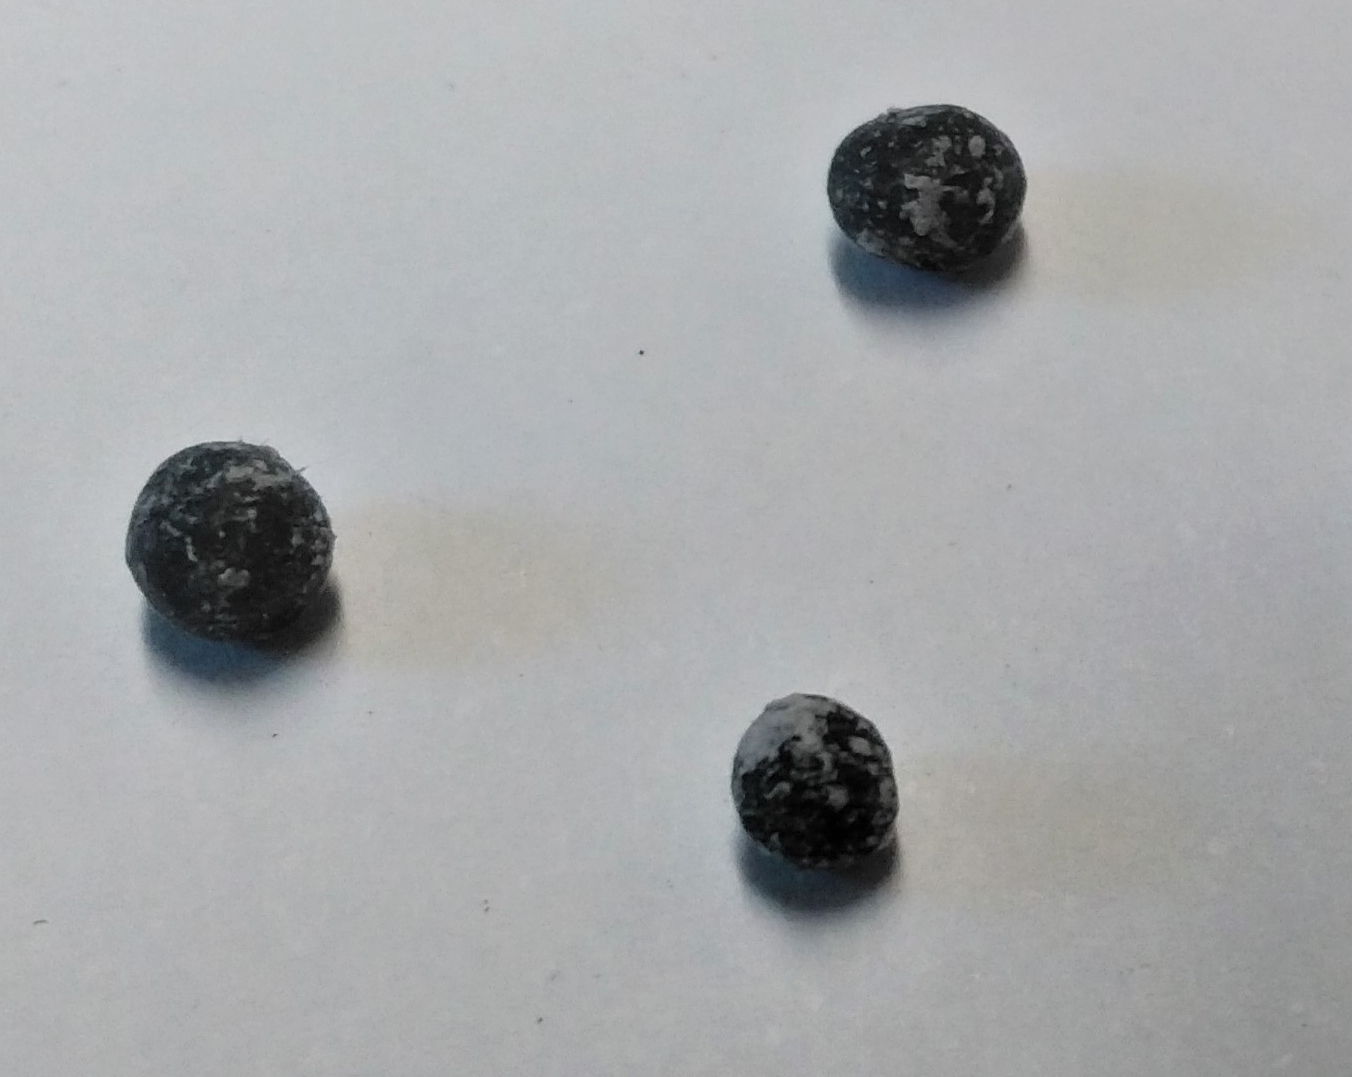
\includegraphics[scale=0.11]{Illustrationen/3-Einleitung/nemacaps.jpg}
	\caption{NemaCaps}
	\label{fig:nemacaps}
\end{wrapfigure}
Die Firma MCC Laboratoire Meiners GmbH ist in der Herstellung von Mikroverkapselungen tätig. Neben der Pharma- und Kosmetikbranche werden Mikroverkapselungen auch in der Landwirtschaft eingesetzt. Für diese Branche entwickelt MCC Laboratoire Meiners GmbH Kapseln, sogenannte NemaCaps, welche in der biologischen Schädlingsbekämpfung eingesetzt werden. Ein NemaCap beinhaltet mehrere tausend Fadenwürmer (Nematoden). Der Kapsel ist ein Schlafmittel beigemischt, sodass die Fadenwürmer schlafend gestellt sind. 

NemaCaps werden im Erdreich eingesetzt. Im Wurzelbereich der zu schützenden Pflanze werden diese platziert. Durch das Begiessen der Pflanze oder Regenfall wird das Schlafmittel verdünnt und die Nematoden werden aktiv. Die Hülle der Kapseln besteht aus \textbf{\textit{XYZ}} welches elastische Eigenschaften besitzt. Dies ist Voraussetzung, dass die Nematoden nach dem Aufwachen die Kapsel durchbrechen können.\newline
In ihrer natürlichen Umgebung angelangt stossen die Fadenwürmer nun zufällig auf Larven von Schädlingen. Gemäss dem Nationalen Forschungsprogramm 68 [nachfolgend NFP 68] (2015) dringen die Nematoden durch die Körperöffnungen der Larven ein (Siehe Abb.  \ref{fig:zyklus_Nematoden}, Punkt 3). im Körper der Larve angelangt, setzen die Fadenwürmer dort Bakterien frei (Punkt 1 in Abb.  \ref{fig:zyklus_Nematoden}). Durch die rapide Vermehrung dieser Mikroben wird die Larve abgetötet. Nach Leillinger und Löckener (2012) vermehren sich die Nematoden im Innern der Larve bis diese komplett aufgezehrt ist. Nun verlassen die Nematoden den Kadaver und befallen weitere Larven. So beginnt der Kreislauf erneut von vorne (Punkt 2 in Abb.  \ref{fig:zyklus_Nematoden}).
\newline

\begin{wrapfigure}[11]{r}{7cm}
	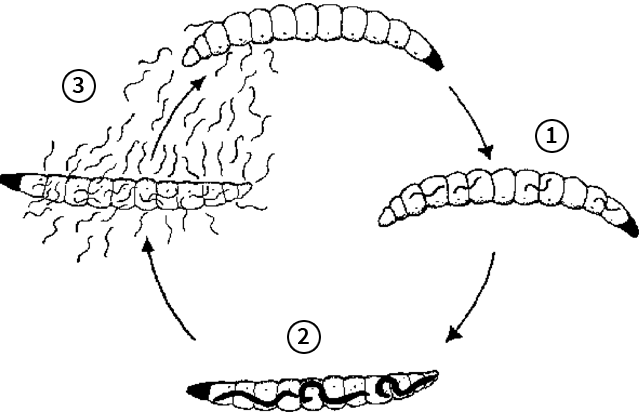
\includegraphics[scale=0.4]{Illustrationen/3-Einleitung/zyklus_nematoden.png}
\caption{Bekämpfung einer Larve durch Nematoden}
\label{fig:zyklus_Nematoden}
\end{wrapfigure}

	
Nematoden bieten speziell in der Bekämpfung gegen Wurzelschädlinge eine wirksame und sichere Alternative zu Pestiziden an. Nach dem NFP 68 (2015) können Pestizide im Wurzelbereich weniger gezielt eingesetzt werden. Die Überlegenheit der Nematoden (im Wurzelbereich?) will man mit NemaCaps nutzen. Durch die Kapselung ist eine gezielte Platzierung sowie Dosierung von Nematoden möglich. Ein weiterer Vorteil der Kapselung ist die verbesserte Handhabung. Die einfache Lagerung sowie Transport von Fadenwürmer wird möglich.  Zusätzlich wird durch die Verwendung des Schlafmittels die Haltbarkeit der Nematoden verlängert. Diese Vorteile unterstreichen das Potential von NemaCaps, der biologischen Alternative von Pestiziden.
